\chapter{ВЫВОД НЕОБХОДИМЫХ УРАВНЕНИЙ}
    \section{Конфигурации модели}
        Для написания алгоритма сканирования в первую очередь необходимо составить математическую модель сканера, то есть вывести соответствующие уравнения, по которым будут рассчитываться координаты точек в сцене. При этом возможно несколько вариантов для вывода необходимых уравнений.
        
        Для расчёта камера представляется пинхол-моделью (pinhole camera model), в которой отверстие соответствует диафрагме и является центром проекции, а экран соответствует получаемому изображению. Начало координат в данной модели располагается в центре проекций -- точке где пересекаются линии проекций точек пространства.
        
        Оси координат направлены следующим образом -- $ Z $ от камеры перпендикулярно плоскости изображения, $ Y $ вниз параллельно короткой стороне кадра, $ X $ вправо параллельно длинной стороне. Таким образом получаем правую систему координат.
        
        \begin{figure}[H]
            \centering
            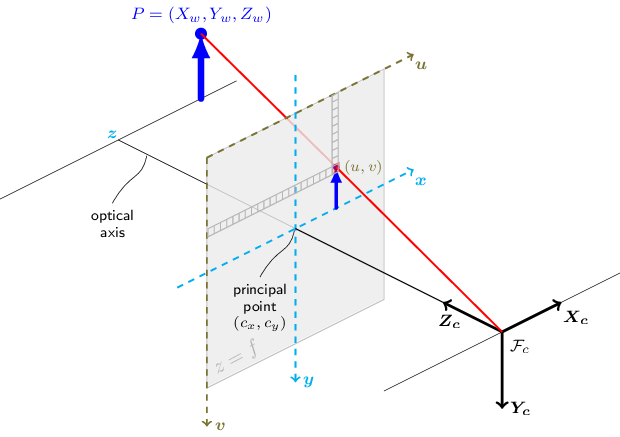
\includegraphics[width=0.5\linewidth]{pinhole_model}
            \caption{Пинхол модель камеры; principal point --- центр изображения, проекция начала координат на плоскость изображения}\label{pic:pinhole_model}
        \end{figure}

        Экран в данной модели может располагаться как между объектом и центром проекции (как показано на рисунке \ref{pic:pinhole_model}), так и за центром проекции. В последнем случае изображение оказывается перевёрнутым.

        \subsection{Условные обозначения}
            $ f $ --- фокусное расстояние камеры в пиксельной мере\\
            $ u,\,v $ --- горизонтальная и вертикальная координаты соответственно в плоскости изображения (пиксели) 
            $ u_0,\,v_0 $ --- координата центра изображения
%            $\Delta u $ --- отклонение лазера от оптического центра на изображении по горизонтальной оси\\
%            $\Delta v$ --- отклонение лазера от оптического центра на изображении по вертикальной оси\\
            
        \subsection{Модель в системе координат принтера}
            Первый расчёт производится в системе координат принтера. Эта модель основывается на реальных размерах сборки и отражает реальную конструкцию модуля. В данном варианте предполагается, что стол -- рабочая поверхность -- находится в плоскости $ XY $, лазер излучает перпендикулярно столу и камера имеет поворот только вокруг оси $ Y $. При этом считается, что лазер не имеет поворота вокруг своей оси.

            \begin{figure}[!ht]\label{pic:first_model}
                \centering
                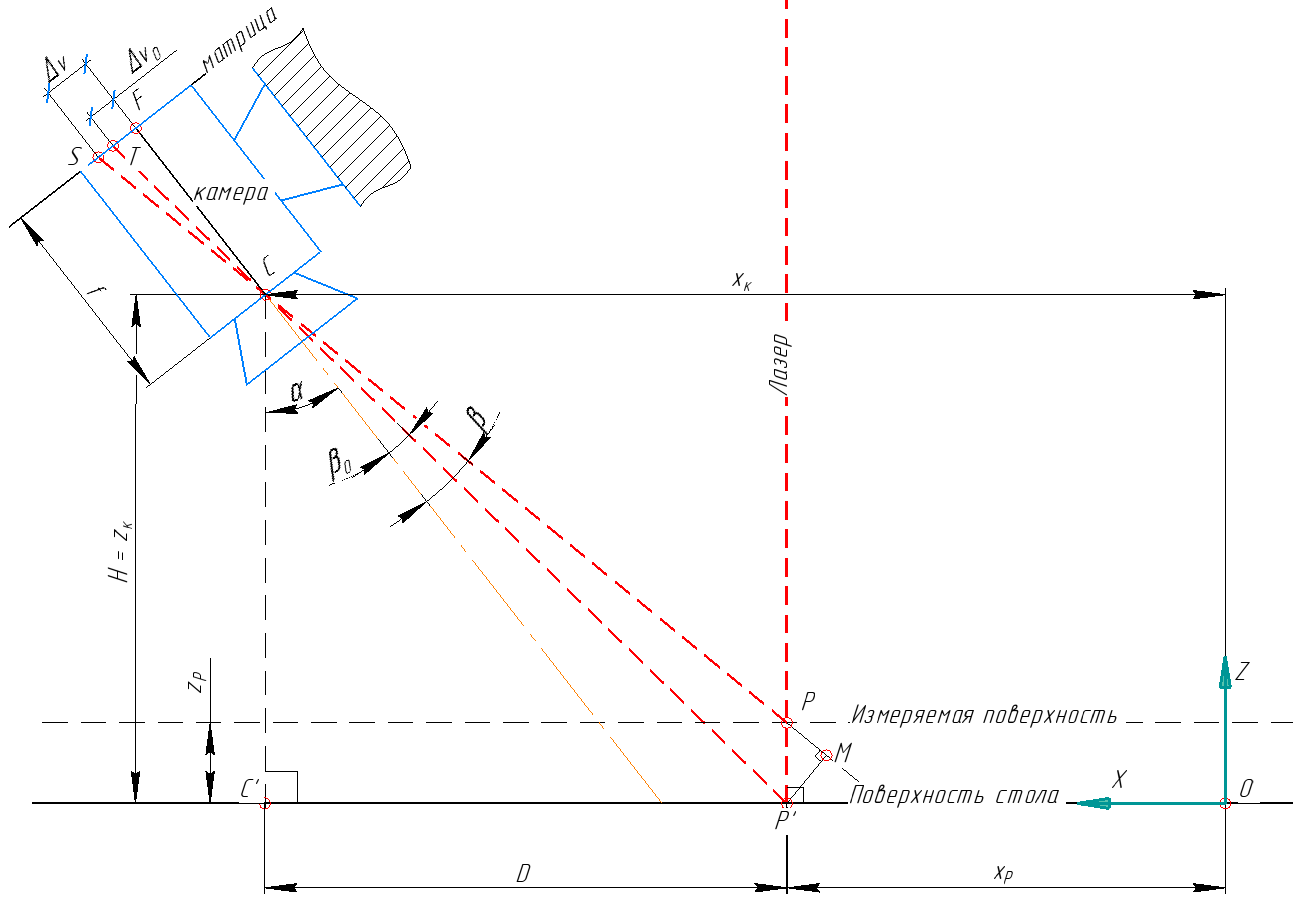
\includegraphics[width=0.75\linewidth]{first_model_xz}
                \caption{Чертёж поясняющий вычисления}
            \end{figure}
            
            \sloppy Необходимо найти уравнения описывающие зависимость координат $ \left(x_P,\,y_P,\,z_P\right) $ точки $ P $ от координат проекции этой точки на плоскость изображения $ \left(u_P, v_P\right) $. Из $ \triangle PP'M $ видно, что
            \begin{equation}
                z_P = \dfrac{P'M}{\cos\angle PP'M}
            \end{equation}
            где $\alpha$ -- угол поворота камеры вокруг оси $ Y $. Далее из $ \triangle CP'M $ очевидно
            \begin{equation}
                P'M = CP'\sin\left(\beta - \beta_0\right)
            \end{equation}
            где $ \beta $ -- произвольный угол падения луча лазера на матрицу, $\beta_0$ -- угол падения луча лазера отражённого от поверхности стола на матрицу. Рассмотрев $ \triangle CP'C' $ можно увидеть, что
            \begin{equation}
                CP' = \dfrac{H}{\cos\left(\alpha + \beta_0\right)}
            \end{equation}
            Подставляя последовательно полученные равенства друг в друга получаем следующее уравнение
            \begin{equation}
                z_P = H\dfrac{\sin\left(\beta - \beta_0\right)}{\cos\left(\alpha + \beta_0\right)\cos\angle PP'M}
            \end{equation}
            нетрудно показать, что
            \begin{equation}
                \cos\angle PP'M = \sin\left(\alpha + \beta\right)
            \end{equation}
            В итоге приходим к уравнению координаты $ z $ точки $ P $, выраженной через углы падения луча лазера на матрицу камеры.
            \begin{equation}
                z_P = H\dfrac{\sin\left(\beta - \beta_0\right)}{\cos\left(\alpha + \beta_0\right)\sin\left(\alpha + \beta\right)}
            \end{equation}
            Расстояние точки $ P $ от камеры при данном методе расчёта константа на всём протяжении линии лазера в виду конструкции и равно расстоянию между камерой и лазером $ C'P' = D $
            \begin{equation}
                D = H\tg\left(\alpha + \beta_0\right)
            \end{equation}
            тогда координата $ x_P $ выражается следующим соотношением
            \begin{equation}
                x_P = x_\text{к} - D = x_\text{к}- H\tg\left(\alpha + \beta_0\right)
            \end{equation}
            Для вывода уравнения координаты $ y_P $ необходимо рассмотреть модуль в проекции на плоскость $ ZY $
            \begin{figure}[H]
                \centering
                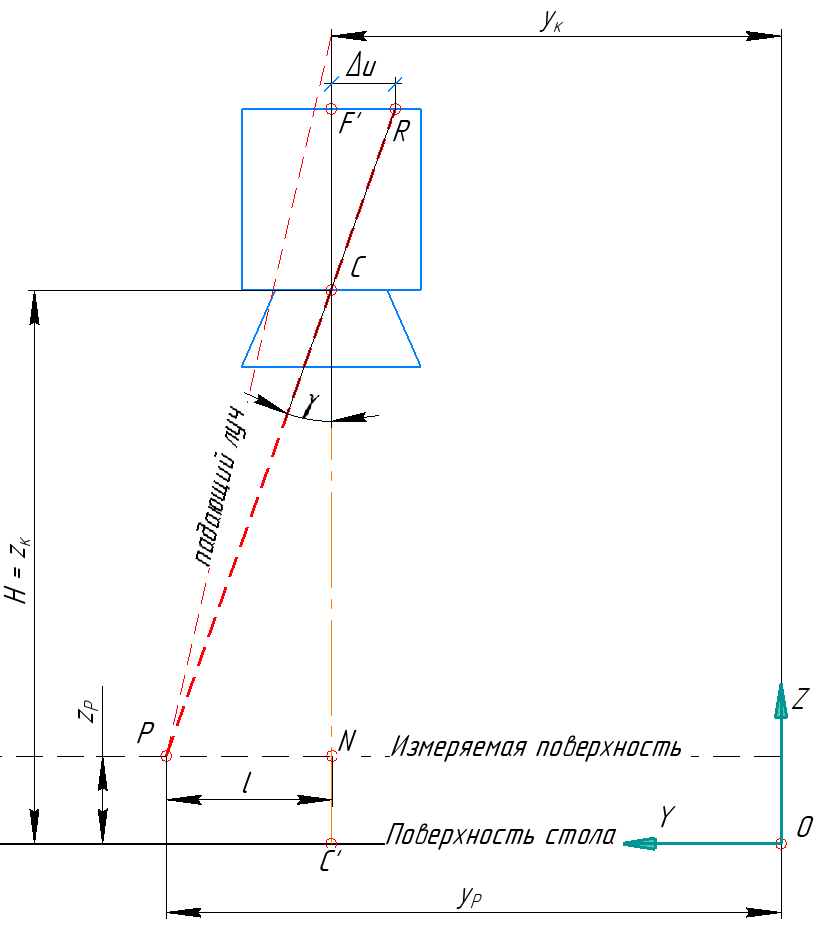
\includegraphics[width=0.5\linewidth]{first_model_yz}
                \caption{Чертёж в проекции на плоскость $ ZY $}
            \end{figure}
            
            При выводе важно помнить, что данный вид -- проекция.
            Из чертежа очевидно, что 
            \begin{equation}
                y_P = y_\text{к} + l
            \end{equation} 
            Из $ \triangle CPN $ легко вывести $ l $
            \begin{equation}
                l = CN\tg\gamma
            \end{equation}
            где $ \gamma $ -- угол падения луча лазера на матрицу в данной проекции. Поскольку $ CN = H - z_P $ можно записать
            \begin{equation}
                y_P = y_\text{к} + (H - z_P)\tg\gamma
            \end{equation}
            Для вывода углов падения $ \beta $ и $ \beta_0 $ рассмотрим $ \triangle CSF$ и $ \triangle CTF $. Очевидно, что
            \begin{equation}
                \begin{aligned}
                    \tg\beta &= \dfrac{\Delta v}{f}\\
                    \tg\beta_0 &= \dfrac{\Delta v_0}{f}
                \end{aligned}
            \end{equation}
            где $ \Delta v = v_P - v_0 $ -- расстояние в пикселях от точки падения луча лазера на матрицу до центра изображения, $ \Delta v_0 = v_{P0} - v_0 $ -- аналогичное расстояние для луча лазера, отражённого от поверхности стола.
            
            Рассмотрев $ \triangle CF'R $ получим значение угла падения в проекции $ ZY $
            \begin{equation}
                \tg\gamma = \dfrac{\Delta u}{CF'} = \dfrac{\Delta u}{f\cos\alpha}
            \end{equation}
            где $ CF' = f\cos\alpha $ -- проекция фокусного расстояния на плоскость $ ZY $.
            Из полученных равенств легко найти значения углов, поскольку величины $ \Delta u $ и $ \Delta v $ известны из изображения с камеры.
            
            Таким образом приходим к следующим уравнениям
            \begin{equation}\label{eq:first_model}
                \begin{aligned}
                    x_P &= x_\text{к}- H\tg\left(\alpha + \beta_0\right)\\
                    y_P &= y_\text{к} + (H - z_P)\dfrac{\Delta u}{f\cos\alpha}\\
                    z_P &= H\dfrac{\sin\left(\beta - \beta_0\right)}{\cos\left(\alpha + \beta_0\right)\sin\left(\alpha + \beta\right)}
                \end{aligned}
            \end{equation}

            Преимущества этой модели:
            \begin{itemize}
                \item $ H $ можно измерять напрямую
                \item рассчитанные значения координат сразу в системе координат принтера
                \item отражает реальную конструкцию сканера
                \item координата $ x $ константа относительно камеры
            \end{itemize}
            
            Недостатки:
            \begin{itemize}
                \item много тригонометрических преобразований
                \item при изменении высоты камеры необходимы новые замеры
                \item большое количество допущений, как следствие много возможностей для ошибок
            \end{itemize}

        \subsection{Модель в системе координат камеры}
            Второй расчёт делается в системе координат связанной с камерой. Эта модель основывается на теоретических величинах и расчёт координат происходит в два этапа. Первый -- расчёт координат относительно камеры, второй -- преобразование в систему координат принтера. В этой модели считается, что лазер не имеет поворота вокруг своей оси, все остальные компоненты могут располагаться произвольно.
            
            Для преобразования между двумя системами координат необходимо знать матрицу поворота системы камеры относительно системы принтера. С помощью пакета opencv можно полностью определить положение камеры в пространстве используя шахматный паттерн.

            Введём следующие определения:\\
            \textit{Рабочая плоскость} --- плоскость перпендикулярная оптической оси камеры и проходящая через точку пересечения оптической оси камеры и луча лазера\\
            \textit{Измеряемая плоскость} --- плоскость, до которой измеряется расстояние 

            \begin{figure}[H]
                \centering
                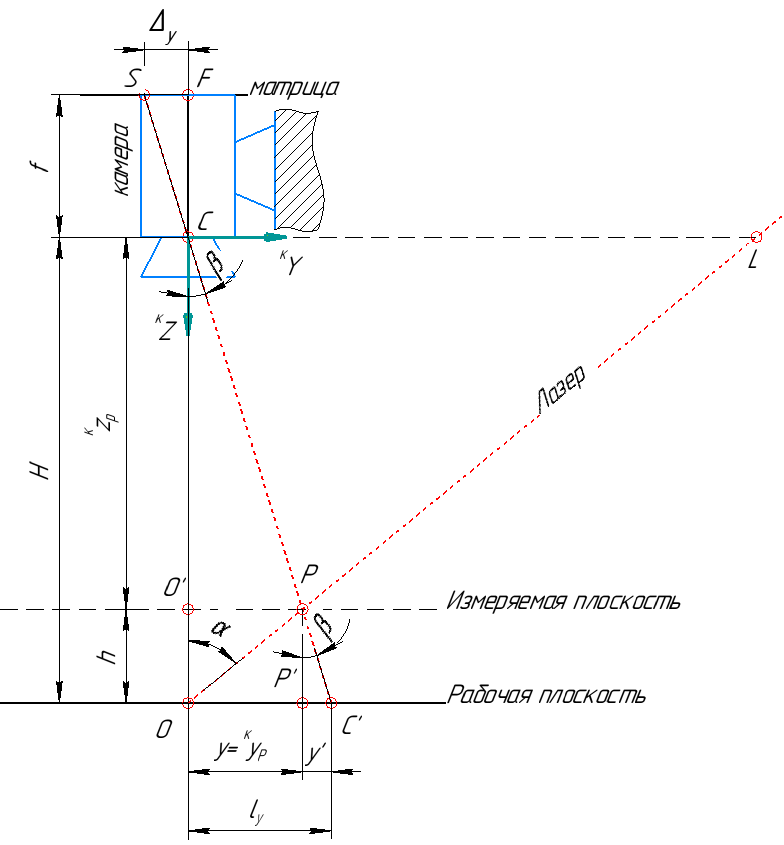
\includegraphics[width=0.75\linewidth]{second_model}
                \caption{Чертёж поясняющий вычисления;
                         $O$ --- точка пересечения оптической оси камеры и луча лазера (плоскости свечения лазера);
                         $C$ --- оптический центр камеры, начало координат СК камеры;
                         $P$ --- точка пересечения луча лазера и измеряемой плоскости;
                         $P'$ --- проекция точки $ P $ на рабочую плоскость;
                         $h$ --- высота измеряемой плоскости над рабочей плоскостью;
                         $l_x,\,l_y$ --- кажущиеся координаты измеряемой точки;
                         $x,\,y$ --- реальные координаты измеряемой точки;
                         $x',\,y'$ --- разность кажущейся и реальной координаты измеряемой точки}
                 \label{pic:second_model}
                 \cbox{ИСПРАВИТЬ ЧЕРТЁЖ}
            \end{figure}
            
            На рисунке \ref{pic:second_model} обозначены следующие размеры:\\
            $ H $ -- рабочая высота, расстояние от оптического центра камеры до рабочей плоскости.\\
            $ \alpha $ -- угол между осями камеры и лазера.
            
            \sloppy Необходимо найти уравнения описывающие зависимость координат $ \left(\kxp,\,\kyp,\,\kzp\right) $ точки $ P $ в системе координат камеры от координат проекции этой точки на плоскость изображения $ \left(u_P,\,v_P\right) $. 
            Из чертежа очевидно, что 
            \begin{equation}
                \kzp = H - h,
            \end{equation} 
            где $ h $ -- высота измеряемой плоскости над рабочей. 
            Рассмотрим треугольники $ \triangle OPC $, $ \triangle OPP' $, $\triangle PCP' $.
            Видно что 
            \begin{equation}
                l_y = y + y',
            \end{equation}
            где $ l_y $ -- кажущаяся координата точки $ P $, $ y = \kyp $ -- реальная координата точки $ P $, $ y' $ -- разность реальной и кажущейся координаты.
            Так как $ PP' = h $ можно записать следующее:
            \begin{equation}
                \begin{aligned}
                    y &= h \tg\alpha\\
                    y' &= h \tg\beta
                \end{aligned}
            \end{equation}
            где $ \beta $ -- угол при вершине $ P $ в треугольнике $ \triangle PCP' $, $ \alpha $ -- угол между оптической осью камеры и осью лазера.
            Также из треугольника $ \triangle COC' $ ясно
            \begin{equation}
                l = H \tg\beta
            \end{equation}
            следовательно
            \begin{equation}
                H\tg\beta = h\left(\tg\alpha+\tg\beta\right)
            \end{equation}
            Зная, что $ h = H - \kzp $ получаем
            \begin{equation}
                \kzp = H \dfrac{\tg\alpha}{\tg\alpha + \tg\beta}
            \end{equation}
            
            Из треугольника $ \triangle CF\cbox{\text{НЕТ БУКВЫ}} $ находим
            \begin{equation}
                \tg\beta = \dfrac{\Delta v}{f},
            \end{equation}
            где $ \Delta v = v_P - v_0 $, $ f $ -- фокусное расстояние камеры.
            В итоге получаем
            \begin{equation}
                \kzp = H \dfrac{\tg\alpha}{\tg\alpha + \frac{\Delta v}{f}}
            \end{equation}
            Далее из $ \triangle C\cbox{\text{НЕТ БУКВЫ}}P $ очевидно, что
            \begin{equation}
                \kyp = \kzp \tg\beta = H \dfrac{\tg\alpha\frac{\Delta v}{f}}{\tg\alpha + \frac{\Delta v}{f}}
            \end{equation}
            аналогично для $ \kxp $
            \begin{equation}
                \kxp = H \dfrac{\tg\alpha\frac{\Delta u}{f}}{\tg\alpha + \frac{\Delta v}{f}}
            \end{equation}
            где $ \Delta u = u_P-u_0 $.
            
            В результате для системы координат камеры получаем:
            \begin{equation}\label{eq:second_model}
                \begin{aligned}
                    \kxp = H\frac{\tg\alpha\frac{\Delta u}{f}}{\tg\alpha+\frac{\Delta v}{f}}\\
                    \kyp = H\frac{\tg\alpha\frac{\Delta v}{f}}{\tg\alpha+\frac{\Delta v}{f}}\\
                    \kzp = H\frac{\tg\alpha}{\tg\alpha+\frac{\Delta v}{f}}
                \end{aligned}
            \end{equation}
            
            Для перевода в систему координат принтера:
            \begin{equation}
                \label{eq:coord_world}
                \begin{pmatrix}
                    x\\y\\z
                \end{pmatrix}
                =
                R
                \begin{pmatrix}
                    \kxp\\ \kyp\\ \kzp
                \end{pmatrix}
                +
                \begin{pmatrix}
                    x_\text{к}\\y_\text{к}\\z_\text{к}
                \end{pmatrix}
            \end{equation}
            
            Преимущества модели:
            \begin{itemize}
                \item отсутствие тригонометрии в расчётах координат
                \item параметры $ H $ и $ \alpha $ фиксированы
                \item меньшее количество допущений
            \end{itemize}
            
            Недостатки модели:
            \begin{itemize}
                \item сложно прямо измерить $ H $ и $ \alpha $, необходим теоретический расчёт
                \item необходима матрица поворота камеры
            \end{itemize}
            
            В этом методе главными параметрами являются высота камеры над рабочей плоскостью и угол между камерой и лазером, но они рассчитываются теоретически и не совпадают с аналогичными из предыдущего метода.
        \subsection{Выбор модели}

    \section{Оценка теоретической погрешности}\label{sec:error}
    
    \section{Калибровка сканера}